%!TEX root = ../Thesis.tex

\chapter{Ergebnisse und Auswertung}
\label{cha:results}

% Screenshots weiterer Straßenabschnitte
% Aufzeigen von Problemen und deren Ursachen
% Mögliche Weiterentwicklungen

Die Stärken, Schwächen und Ergebnisse des entwickelten Algorithmus werden im nachfolgenden Kapitel
zusammengefasst, diskutiert und ausgewertet. Es wird zuerst abschnittsweise auf die drei primären Schritte
des Verfahrens eingegangen. Anschließend werden Beispiele erkannter Fahrspuren aufgeführt.

\section{Evaluierung der Datenvorverarbeitung}

% Sehr wichtig für zuverlässige Funktionsweise der nachfolgenden Schritte.
% Kurz: Ziele (Bereinigung von Ausreißern, Reduktion der Komplexität)
% Funktioniert gut: Entfernt stehende oder unterbrochene Trajektorien, außerdem einzelne Ausreißer aufgrund von Tracking Fehlern 
% Beispiel Heilbronner Straße (Raw | filtered)

% Problematisch: Trajektorien einer Spur enden alle auf unterschiedlichen Höhen (--> Horizont)
% Algorithmus aus XXX würde viele (im Schlimmsten Fall alle) Trajektorien entfernen
% Beispiel Steinheim (RAW | Trajektorien an Horizont | Trimmed Trajs)
% Verweiß 

Die Datenvorverarbeitung ist ein wichtiger Teilschritt bei der Erkennung von Fahrspuren. Nur wenn aus
den Roh-Trajektorien die meisten Defekte entfernt wurden, können die nachfolgenden
Schritte zuverlässig funktionieren. Die meisten Defekte in den Roh-Trajektoriedaten werden durch stehende
Fahrzeuge und fehlerhafte oder unterbrochene Fahrzeugverfolgungen verursacht. Die angewandten Schritte zur
Entfernung der Anomalien sind in Abschnitt \ref{sec:realisation_preprocessing} beschrieben.

Dass die Entfernung von Ausreißern funktioniert, wurde bereits zum Teil in Abbildung
\ref{fig:real_result_2nd_Prepro} anhand des Neckartor-Trajaktoriedatensatzes gezeigt.
In Abbildung \ref{fig:results_prePro_heilbronner} sind nun die Trajektorien eines weiteren Datensatzes dargestellt,
welcher von der Heilbronner-Straße in Stuttgart stammt. 

\begin{figure}[H]
    \centering
    \subfloat[]{{
        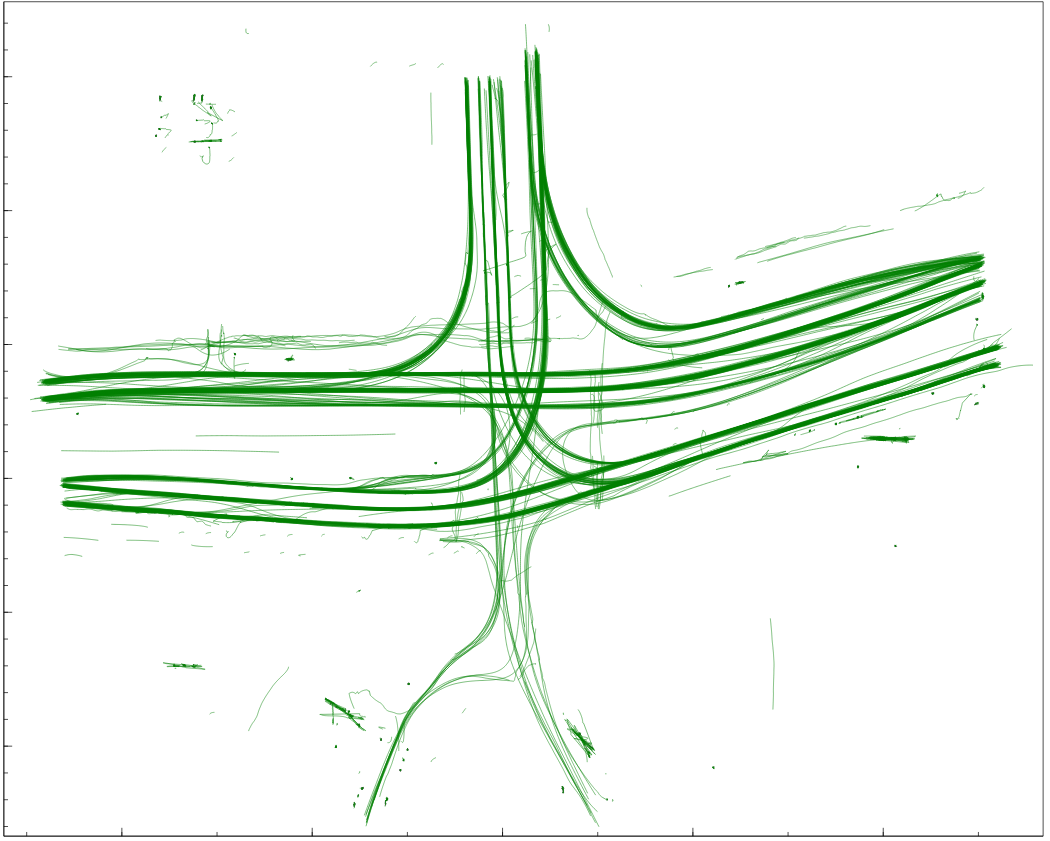
\includegraphics[align=c, width=0.33\linewidth]{resources/img/results/Heilbronner/rawTrajectories}
    }}
    \qquad \qquad
    \subfloat[]{{
        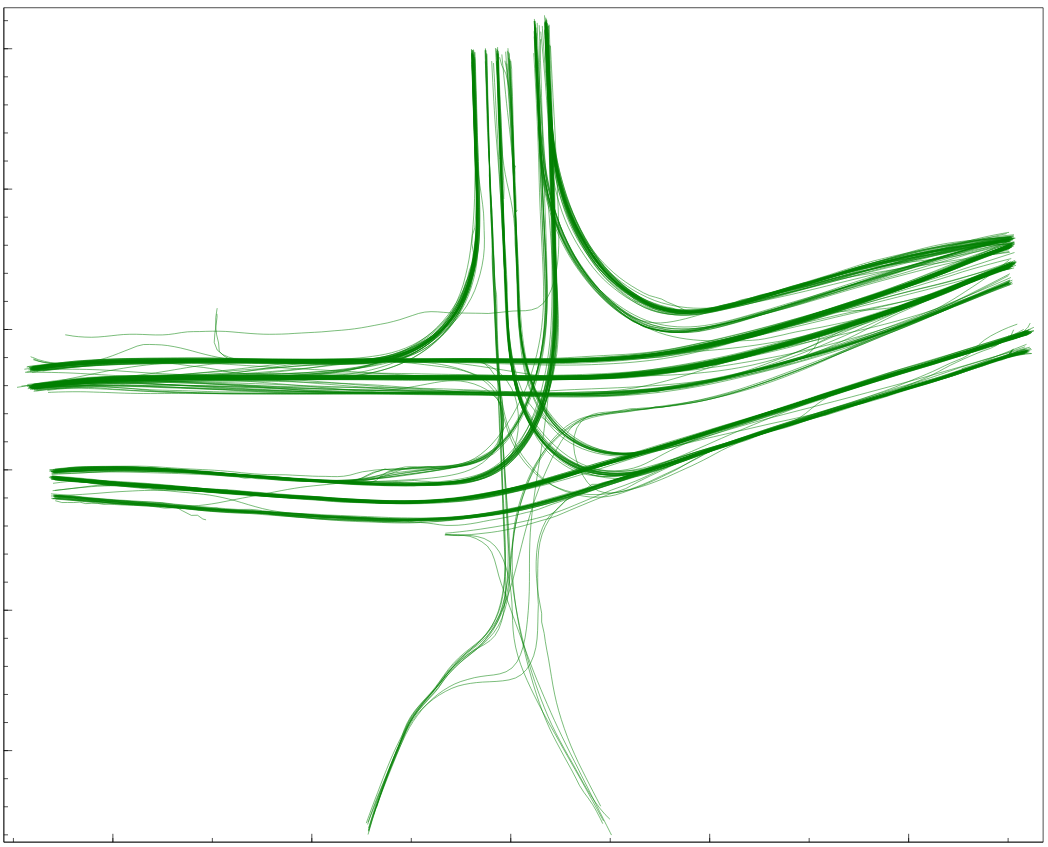
\includegraphics[align=c, width=0.33\linewidth]{resources/img/results/Heilbronner/preProTrajs}
    }}
    \caption{Ergebnis Vorverarbeitung Heilbronner-Straße}
    \label{fig:results_prePro_heilbronner}
\end{figure}

Die zwei obigen Plots zeigen gut, dass die vielen in a) vorkommenden Defekte entfernt wurden. Von den
circa 1050 Roh-Trajektorien im ursprünglichen Datensatz bleiben nach der Vorverarbeitung etwa 450 intakte
Bewegungsbahnen übrig. Die Mehrzahl der Defekte in diesem Fall stammt von fehlerhaften Objekterkennungen
und unterbrochener Fahrzeug-Detektionen, welche aufgrund der Verdeckung von Fahrspuren durch Bäume entstehen.

Ein problematisches Verhalten des Vorverarbeitungsschrittes wurde beim Testen der Spurerkennung anhand eines
Datensatzes aus Steinheim deutlich. In Abbildung \ref{fig:results_horizon_problem} a) ist der
untersuchte Straßenabschnitt dargestellt.

\begin{figure}[H]
    \centering
    \subfloat[]{{
        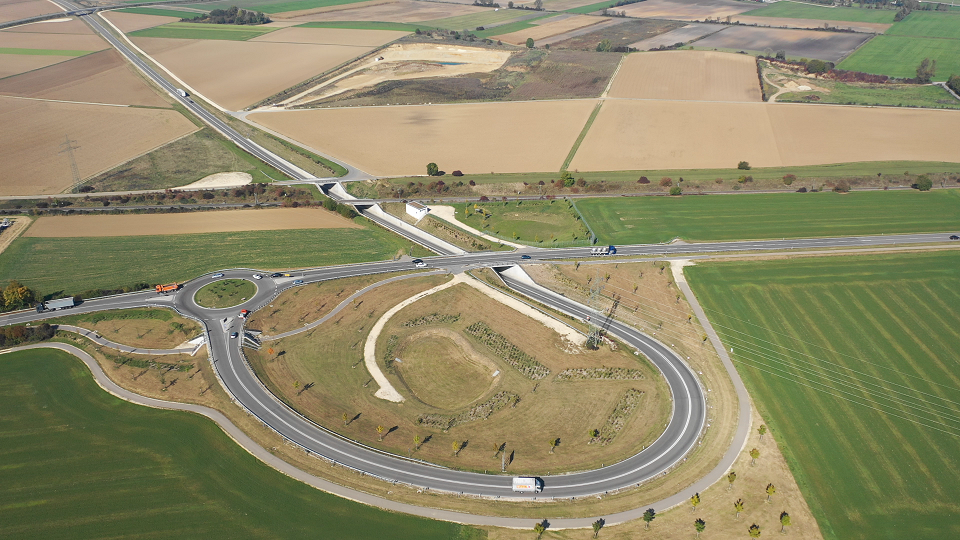
\includegraphics[align=c, width=0.35\linewidth]{resources/img/results/Steinheim/steinheim}
    }}
    \qquad \qquad \qquad
    \subfloat[]{{
        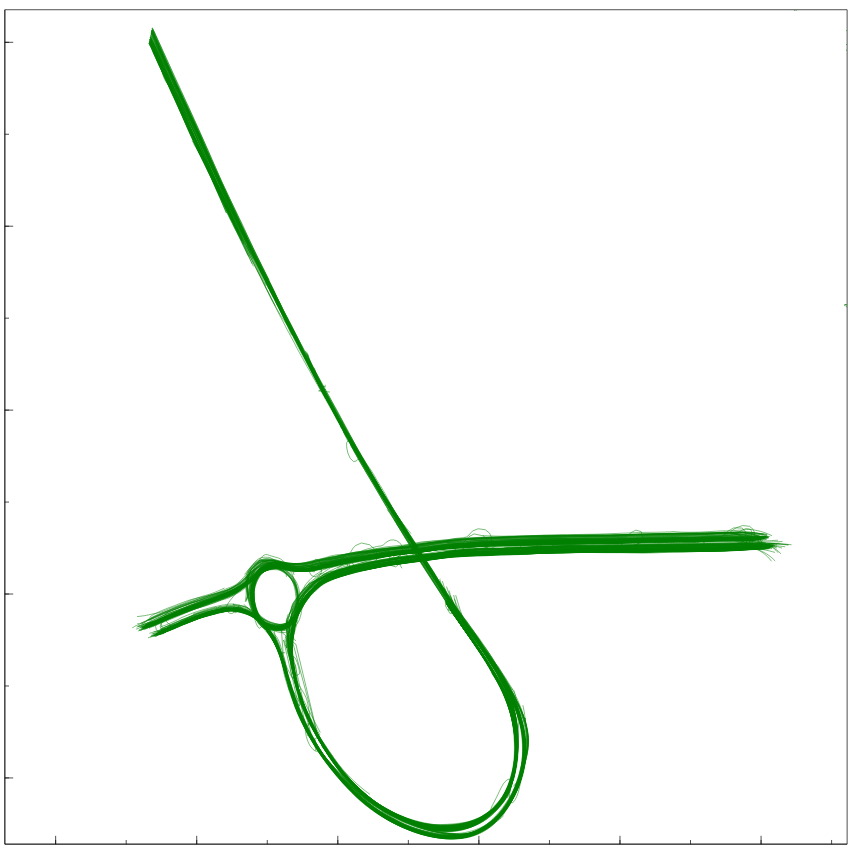
\includegraphics[align=c, width=0.25\linewidth]{resources/img/results/Steinheim/preProTrajs_cut}
    }}
    \caption{Straßenausschnitt Steinheim a), gekürzte Trajektorien b)}
    \label{fig:results_horizon_problem}
\end{figure}

Kritisch an dieser Aufnahme ist, dass die Fahrzeuge, welche sich auf der oben linkes startenden Fahrbahn bewegen,
am Anfang beziehungsweise Ende ihrer Fahrt sehr klein sind. Da die Fahrzeuge in einer Aufnahme ab einer gewissen Größe
nurnoch sehr unzuverlässig detektiert werden, brechen die Trajektorien in diesem Fall auf sehr
unterschiedlichen Höhen ab.
Problematisch ist nun, dass der in Abschnitt \ref{sec:real1_remove_broken_trajectories} beschriebene Algorithmus
zur Entfernung unterbrochener Trajektorien, aufgrund der stark variierenden Start- und End-Positionen,
auch die meisten Trajektorien auf der nach hinten verlaufenden Fahrbahn entfernt und somit die Spuren nicht erkannt werden können.

Da die Fahrzeuge im Bereich des Horizonts nur unzuverlässig erkannt werden, ist auch eine Fahrverhaltensanalyse
mithilfe von Fahrspuren hier wenig sinnvoll. Es wurde daher entschieden dem Anwender die Möglichkeit zu geben, eine
Horizont-Linie zu definieren. In einem ersten Vorverarbeitungsschritt werden alle Trajektorie-Punkte oberhalb dieser
Linie entfernt. Das Ergebnis dieses Verfahrens ist in Abbildung \ref{fig:results_horizon_problem} b)
dargestellt. Dank der Beschneidung der Trajektorien bleiben diese in den nachfolgenden Verarbeitungsschritten
erhalten und es können Spuren im gewünschten Abschnitt erkannt werden.

\section{Evaluierung der Clusteranalyse}

\begin{figure}[H]
\centering
    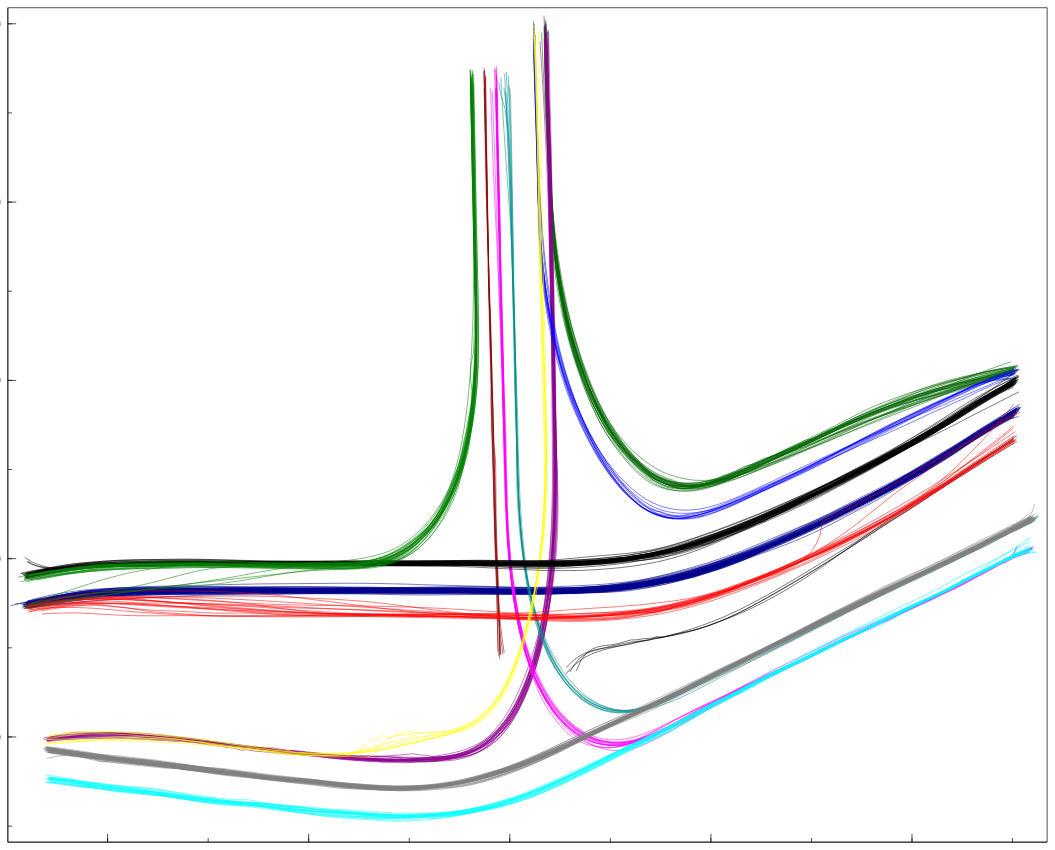
\includegraphics[width=0.38\linewidth]{resources/img/results/Heilbronner/filteredClusters}
\caption{Trajektorie-Cluster Heilbronner Straße}
\label{fig:results_clusters_heilbronner}
\end{figure}

\begin{figure}[H]
    \centering
    \subfloat[]{{
        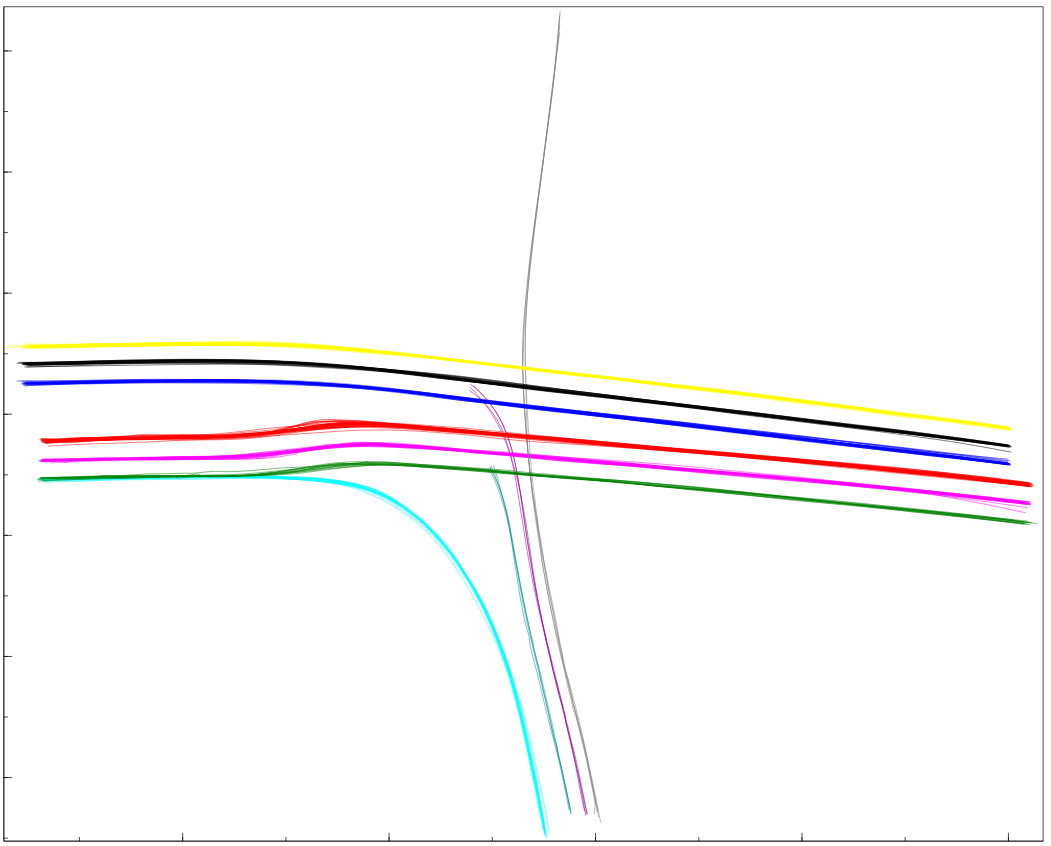
\includegraphics[align=c, width=0.35\linewidth]{resources/img/results/Neckartor/filteredClusters1}
    }}
    \qquad \qquad
    \subfloat[]{{
        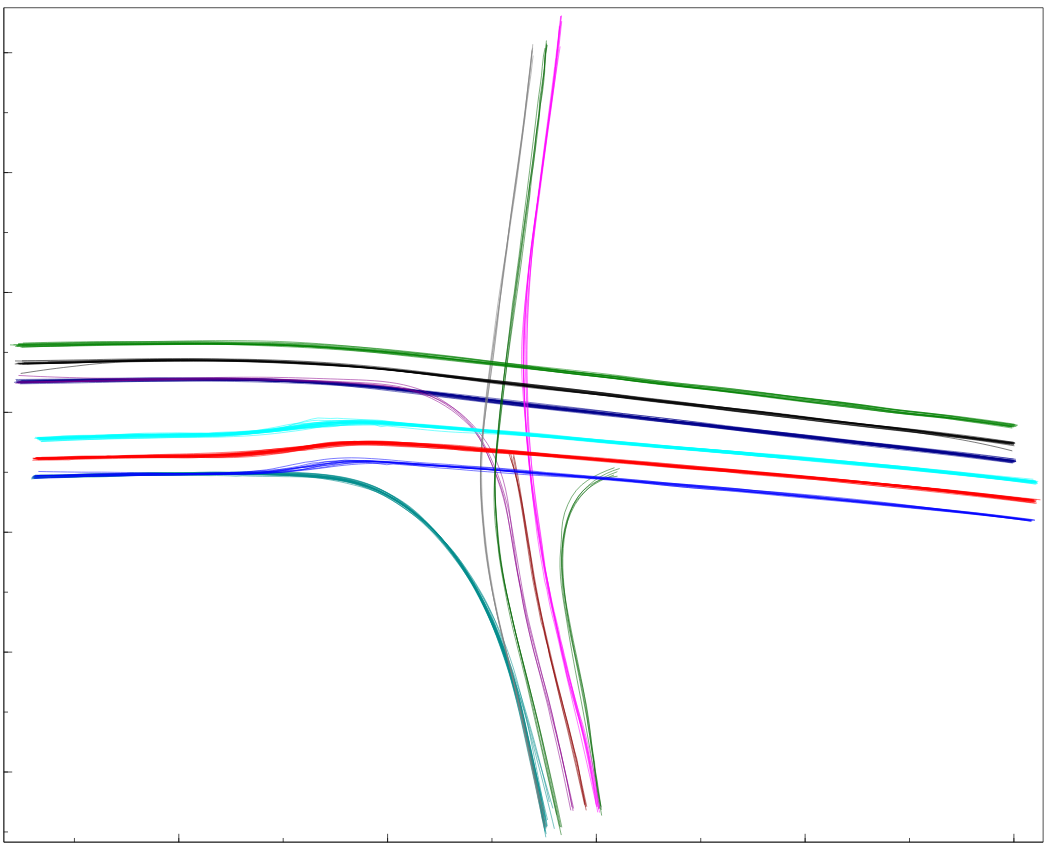
\includegraphics[align=c, width=0.35\linewidth]{resources/img/results/Neckartor/filteredClusters2}
    }}
    \caption{Trajektorie-Cluster Neckator-Kreuzung}
    \label{fig:results_clusters_neckartor_filtered}
\end{figure}

\section{Evaluierung der Spur-Geometrie Bestimmung}

\section{Beispiele erkannter Fahrspuren}
